% Regression predictions input and phys.
\begin{figure}[hp]
    \begin{subfigure}[b]{\linewidth}
    	\centering
        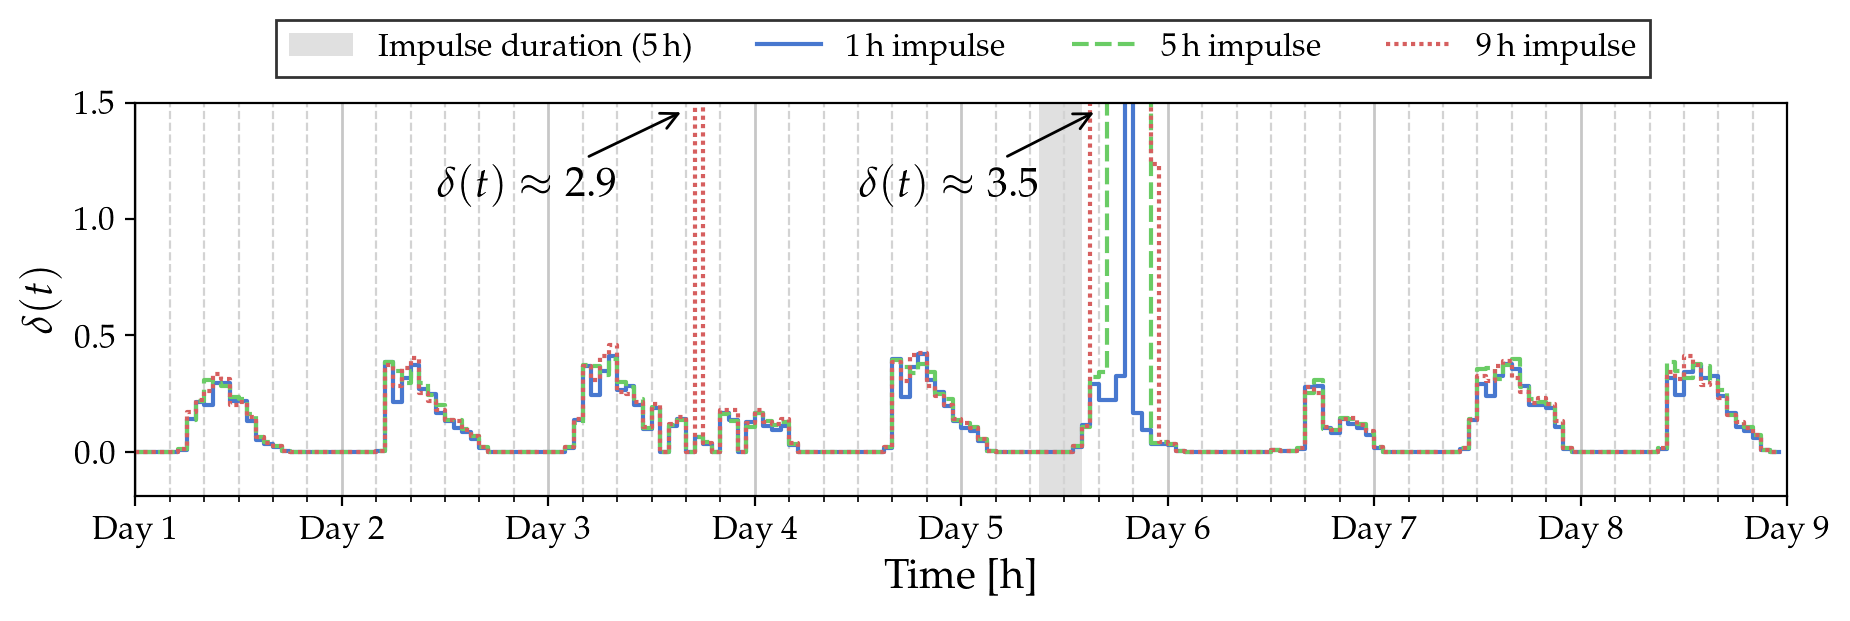
\includegraphics[width=\linewidth,keepaspectratio]{img/hydroshoot_instability_divergence.png}
        \caption{HydroShoot: Reservoir divergence $\delta(t)$ in various experiments with impulse amplitude \SI{0}{\watt\per\square\meter}.}
    	\label{fig:hydroshoot-instability-divergence}
	\end{subfigure}
	\vskip\baselineskip
	\begin{subfigure}[b]{\linewidth}
	    \centering
        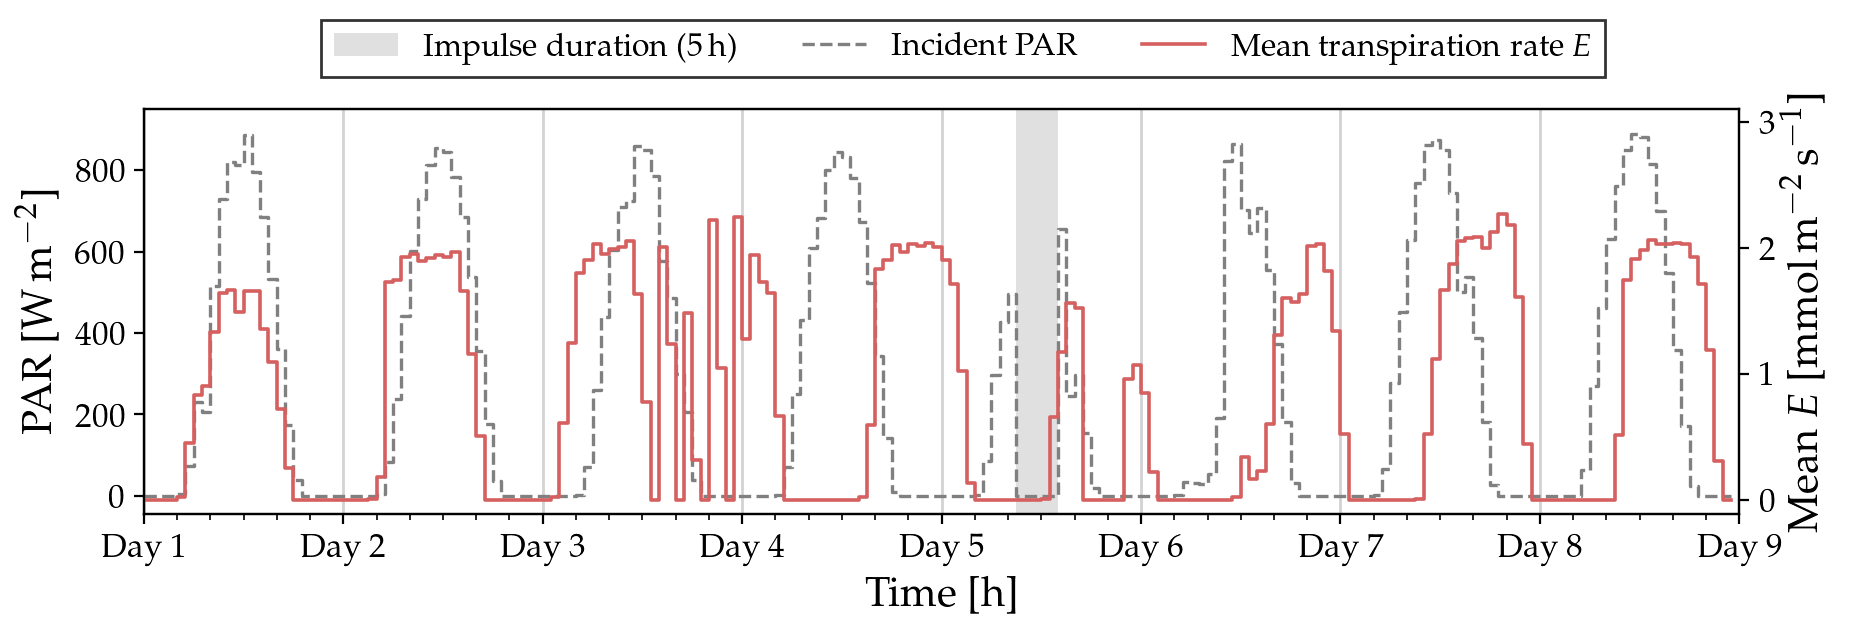
\includegraphics[width=\linewidth,keepaspectratio]{img/hydroshoot_instability_behavior.png}
        \caption{HydroShoot: Input data and modeled transpiration rate from an impulse experiment with length \SI{5}{\hour}.}
    	\label{fig:hydroshoot-instability-behavior}
	\end{subfigure}
	\caption[Two figures highlighting unstable behavior observed in the HydroShoot \acrshort{fspm}.]
        	{Two figures highlighting unstable behavior observed in the HydroShoot \acrshort{fspm}.
        	(\subref{fig:hydroshoot-instability-divergence}) 
	            Reservoir divergence $\delta(t)$ in various experiments with impulse amplitude \SI{0}{\watt\per\square\meter}.
                Under all circumstances, a cyclical pattern of reservoir divergence emerges.
        	(\subref{fig:hydroshoot-instability-behavior}) 
        	    Input data and modeled transpiration rate $E$ from an impulse experiment with length \SI{5}{\hour}.
        	    The superposition of the data reveals a shifting misalignment between the diurnal pattern of incident PAR and the consequent transpiration rate.
        	}
	\label{fig:hydroshoot-instability}
\end{figure}
